\documentclass[12pt]{article}

\usepackage{blindtext}
\usepackage{graphicx}
\usepackage{subcaption}
\usepackage{url}
\usepackage{fixltx2e}

%\usepackage[top=2cm, bottom=2cm, left=2cm, right=2cm]{geometry}
%\usepackage{subcaptions}

\pagenumbering{gobble}

\begin{document}

\title{carica e scarica di un condensatore}
\author{Ionut Cicio 3Binf.}
\date{31-01-2020}

\maketitle

\section*{Obiettivo}
Dimostrare e spiegare il funzionamento di carica e di scarica di un condensatore,
simulando i due circuiti su qucs, ed elaborando i grafici risultanti dalla simulazione.

\section*{Strumenti}
qucs versione 0.0.19 (\url{http://qucs.sourceforge.net/})

\section*{Spiegazione teorica}

\subsection*{definizione}
Il condensatore (\textit{"capacitor"} in inglese) e' un componente elettronico che ha la capacita' di immagazzinare energia sotto forma di campo elettrostatico. \\
Tale energia, nel caso di un condensatore ideale, viene conservata all'infinito.\\
(nel caso reale, essendo che tutto e' fatto di materiale, tutto ha una resistenza, per cui, anche se molto lentamente, il condensatore si scarica)

\subsection*{composizione}
Il condensatore e' composto da due conduttori detti armature, o piatti, separati da un materiale isolante detto dielettrico. \\
In particolare, quando viene applicata una tensione ai capi delle armature, le piccole cariche all'interno del dielettrico \textit{"ruotano"} in modo da allinearsi con con il campo elettrico.
Cio' e dimostrabile dal fatto che il condensatore si riscalda, fenomeno dovuto all'attrito generato dalla rotazione di queste cariche. \\

Su ogni condensatore vengono indicati la capacita' e la tensione 
massima supportata (figura 1) (infatti, se viene applicata una tensione troppo alta, gli elettroni del dielettrico raggiungono la banda di conduzione, per cui il dielettrico viene attraversato da una carica \textit{distruptiva}, e il condensatore esplode; anche nel caso in cui il dielettrico
sopravvive, come nei condensatori ad aria, le armature si possono comunque fondere). \\

Esistono diversi tipi di condensatori (figura 4): ceramici, a poliestere, variabili, ed elettrolitici; esistono piccoli condensatori che si attaccano direttamente all PCB (figura 2, C3). In particolare c'è un discorso da fare sui condensatori elettrolitici: oltre ad essere polarizzati (quindi vanno inseriti nel verso corretto, altrimenti possono rompersi), essendo condensatori in genere molto capienti, contenenti acido, hanno una \textit{"valvola"} nella parte superiore, per rilasciare la pressione nel caso di tensioni troppo elevate, in modo da non esplodere (figura 3). \\ 

\begin{figure}[h!]
  \centering
  \begin{subfigure}[b]{0.25\linewidth}
    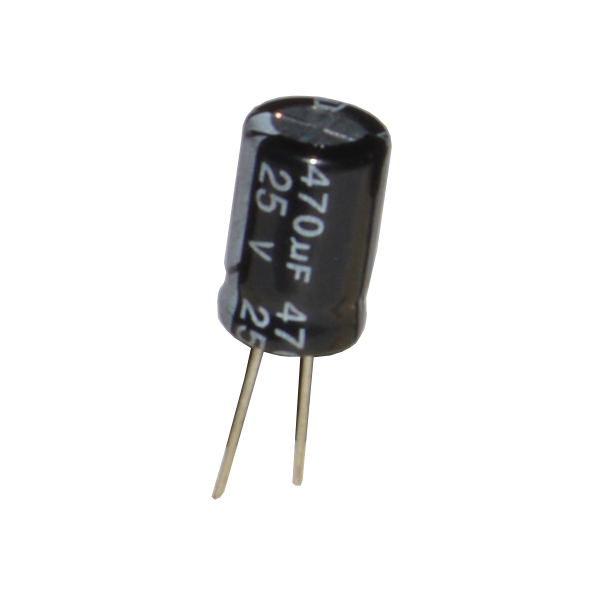
\includegraphics[width=\linewidth]{data/condensatore-reale.jpg}
    \caption*{figura 1}
  \end{subfigure}
  \begin{subfigure}[b]{0.25\linewidth}
    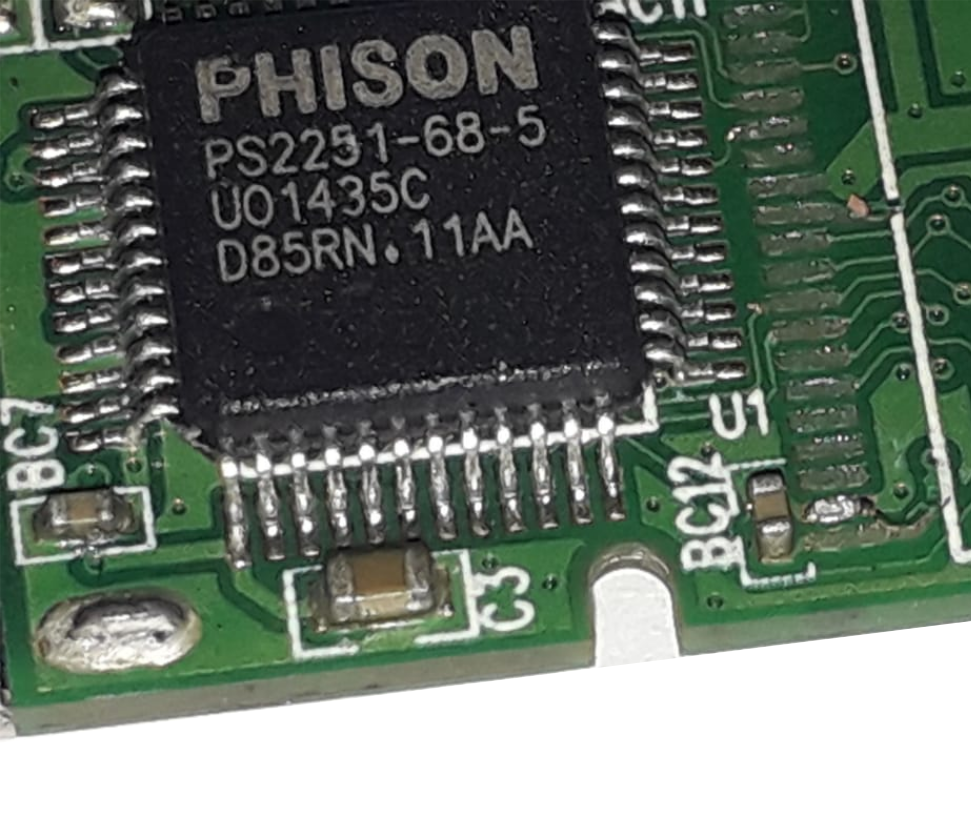
\includegraphics[width=\linewidth]{data/PCB-capacitor.png}
    \caption*{figura 2}
  \end{subfigure}
  
  \begin{subfigure}[b]{0.25\linewidth}
    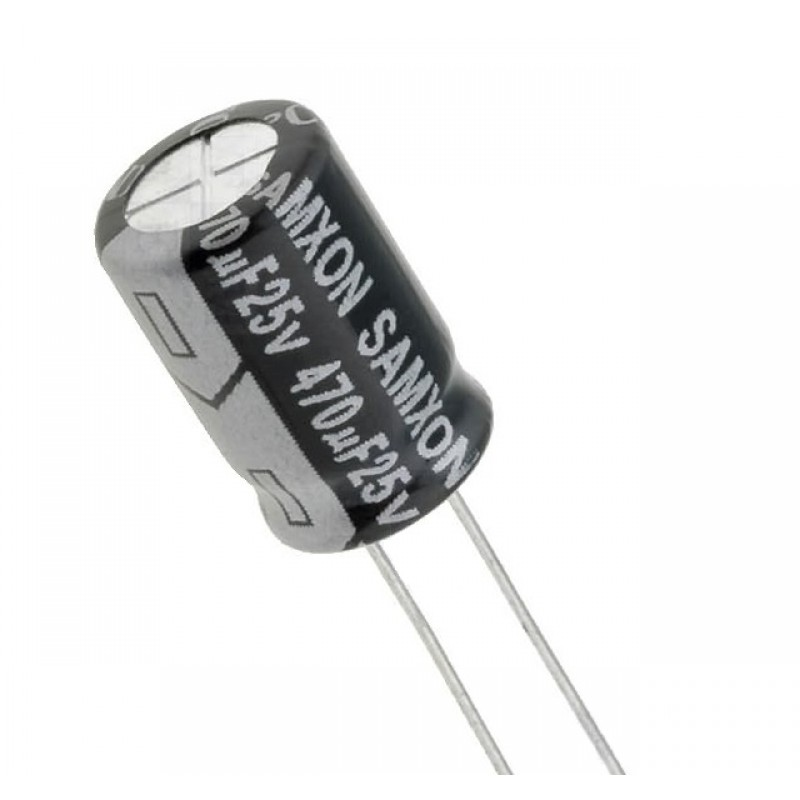
\includegraphics[width=\linewidth]{data/condensatore-elettrolitico-valvola.jpg}
    \caption*{figura 3}
  \end{subfigure}
  \begin{subfigure}[b]{0.25\linewidth}
    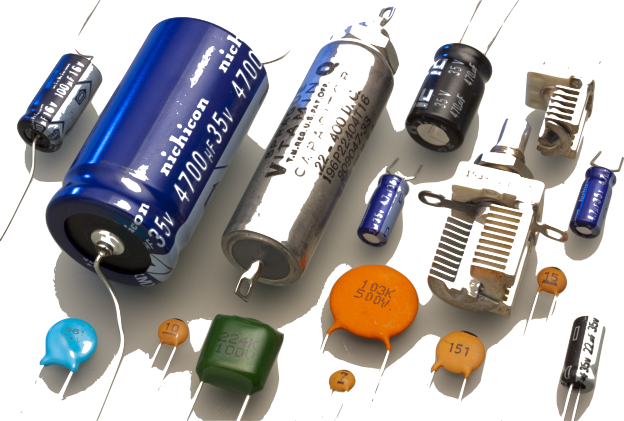
\includegraphics[width=\linewidth]{data/capacitors-types.png}
    \caption*{figura 4}
  \end{subfigure}
\end{figure}

\subsection*{formule relative al condensatore}
Per determinare la capacita' effettiva del condensatore, basandoci sulla sua composizione fisica e chimica si usa la formula 
%\begin{equation}
%C=\varepsilon\textsubscript{0}\varepsilon\textsubscript{r}\frac{S}{d}
%\end{equation}
C = $\varepsilon$\textsubscript{0}$\varepsilon$\textsubscript{r}$\frac{S}{d}$
dove $\varepsilon$\textsubscript{0} indica la 
\textit{costante dielettrica nel vuoto} (4$\pi\cdot$10\textsuperscript{-12}),
dove $\varepsilon$\textsubscript{r} indica la \textit{costante dielettrica relativa al materiale},
S la superficie sovrapposta delle armature e d la distanza fra le armature. \\

Un altro dei parametri fondamentali quando si considera il condensatore all'interno
del circuito e' il tempo di carica, determinabile con t = 5$\tau$, dove $\tau$, 
che indica la \textit{"velocità"} di carica del condensatore, e' dato dal prodotto fra 
la capacita' C del condensatore e la resistenza totale R, vista dal condensatore: $\tau$ = RC. \\

La curva di carica e di scarica del condensatore e' di tipo esponenziale, avendo
Q(t) = $\varepsilon$C(1 - e\textsuperscript{-t/$\tau$}).
Sapendo che Q = CV $\Rightarrow$ V = $\frac{Q}{C}$, si avrà \\
V(t) = $\varepsilon$(1 - e\textsuperscript{-t/$\tau$}). \\

Anche la percentuale di carica del condensatore in funzione al tempo e' di tipo esponenziale
avendo infatti x = 100(1 - e\textsuperscript{-t/$\tau$}), dove x indica la percentuale di carica.

\newpage

\section*{circuito di carica}

\begin{figure}[h!]
  \centering
  \begin{subfigure}[b]{0.3\linewidth}
    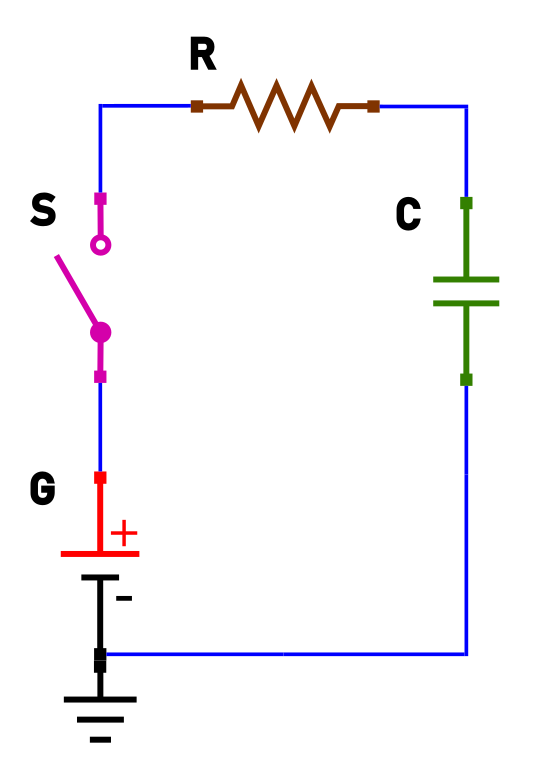
\includegraphics[width=\linewidth]{data/carica-open.png}
  \end{subfigure}
  \begin{subfigure}[b]{0.3\linewidth}
    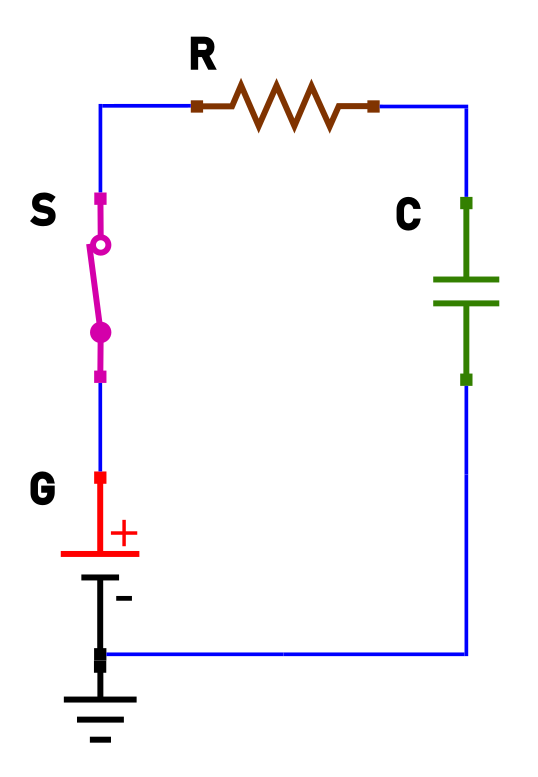
\includegraphics[width=\linewidth]{data/carica-closed.png}
  \end{subfigure}
  \begin{subfigure}[b]{0.347\linewidth}
    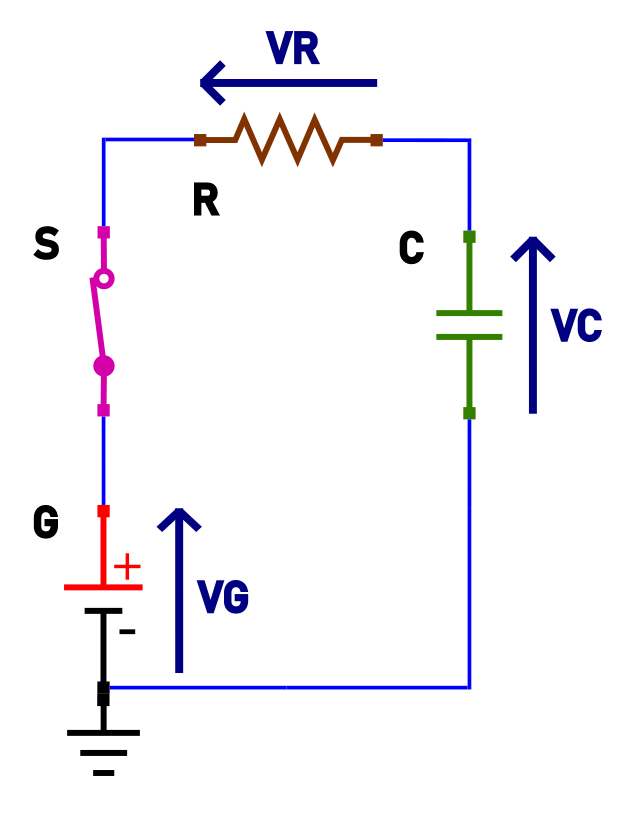
\includegraphics[width=\linewidth]{data/carica-tensioni.png}
  \end{subfigure}
\end{figure}

Il circuito progettato per la carica del condensatore nella prima figura si possono individuare G = 12V, R = 10k$\Omega$, C = 33$\mu$F. Asserito ciò, si può determinare che 
$\tau$ = 1$\cdot$10\textsuperscript{4}$\cdot$ 33$\cdot$10\textsuperscript{-5} $\Rightarrow$ $\tau$ = 0.33, avendo infine t = 1.65 . \\
In particolare l'interruttore S verrà chiuso dopo 1 secondo, quindi si può ipotizzare che il condensatore sarà completamente carico a 2.65 secondi della simulazione, quindi una simulazione di 4 secondi e' più che sufficiente per far raggiungere al condensatore una carica del 99\% (il condensatore, al livello teorico infatti, ci mette un tempo $\infty$ per caricarsi al massimo)


\subsection*{grafici carica}
\begin{figure}[h!]
  \centering
  \begin{subfigure}[b]{0.49\linewidth}
    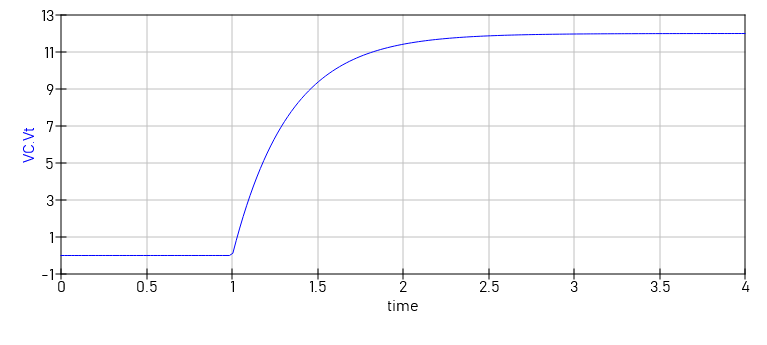
\includegraphics[width=\linewidth]{data/carica-VC.png}
    \caption*{grafico VC}
  \end{subfigure}
  \begin{subfigure}[b]{0.49\linewidth}
    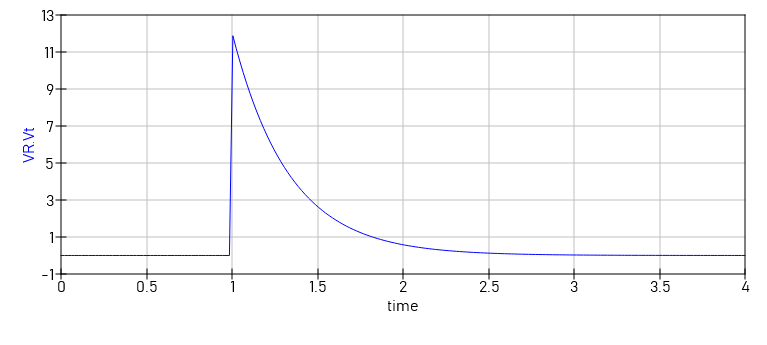
\includegraphics[width=\linewidth]{data/carica-VR.png}
    \caption*{grafico VR}
  \end{subfigure}
  
  %\begin{subfigure}[b]{0.45\linewidth}
  %  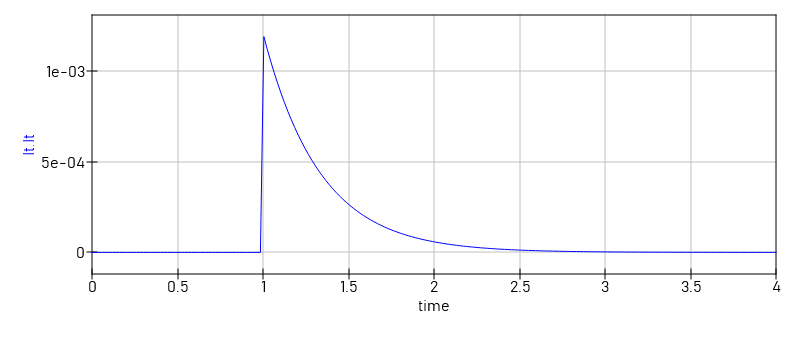
\includegraphics[width=\linewidth]{data/carica-IT.png}
  %\end{subfigure}
\end{figure}
Dai grafici risultanti dalla simulazione possiamo notare i risultati ipotizzati corrispondono a quelli effettivi: l'andamento di VC e' di tipo esponenziale, oltretutto si può notare che VR scende in modo esponenziale, fenomeno che si può spiegare con la legge di Kirchhoff sulle maglie: VG = VR + VC, quindi, se VC aumenta, perché l'equazione sia vera, VR deve scendere. \\
%\enlargethispage{\baselineskip}
\begin{figure}[h!]
  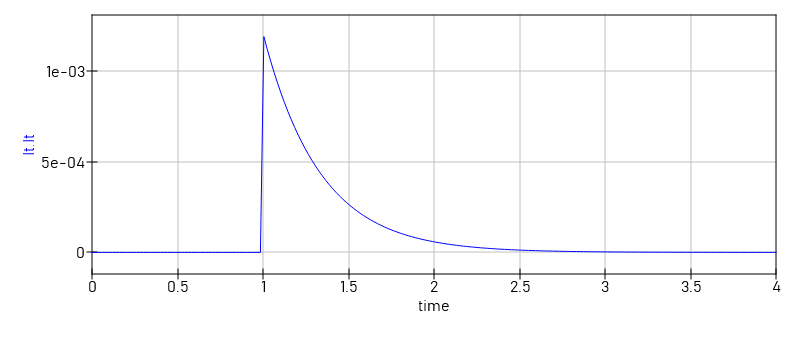
\includegraphics[width=\linewidth]{data/carica-IT.png}
  \caption*{andamento corrente carica}
\end{figure}

Come si può ben notare l'andamento della corrente totale scende mentre il condensatore si carica. Questo risultato è semplice da spiegare: I = $\frac{V}{R}$, e, sapendo che la tensione VR scende con il caricarsi del condensatore, anche la corrente (inizialmente 1.2 mA) diminuisce in maniera esponenziale. 

\begin{figure}[h!]
  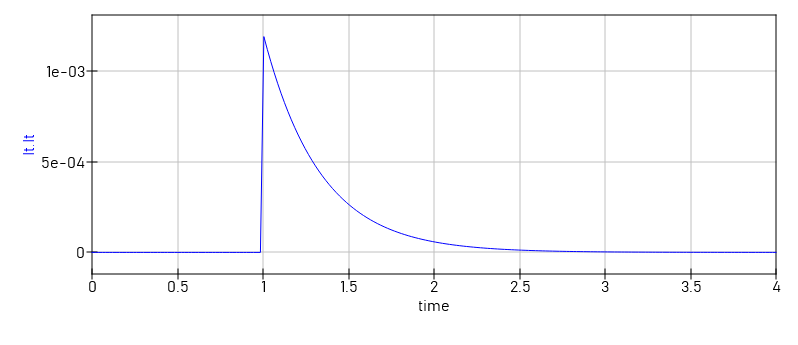
\includegraphics[width=\linewidth]{data/scarica-IT.png}
  \caption*{andamento corrente scarica}
\end{figure}

Anche nella scarica la corrente subisce lo stesso fenomeno.


\newpage
\section*{circuito di sarica}

\begin{figure}[h!]
  \centering
  \begin{subfigure}[b]{0.3\linewidth}
    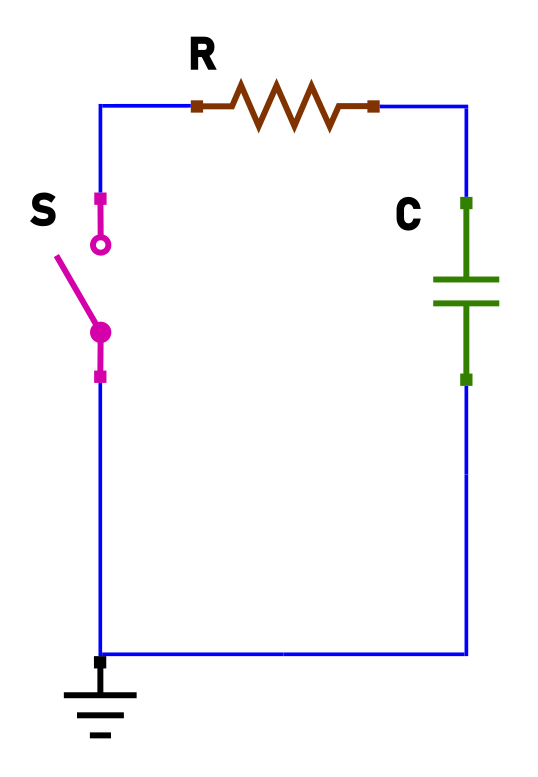
\includegraphics[width=\linewidth]{data/scarica-open.png}
  \end{subfigure}
  \begin{subfigure}[b]{0.3\linewidth}
    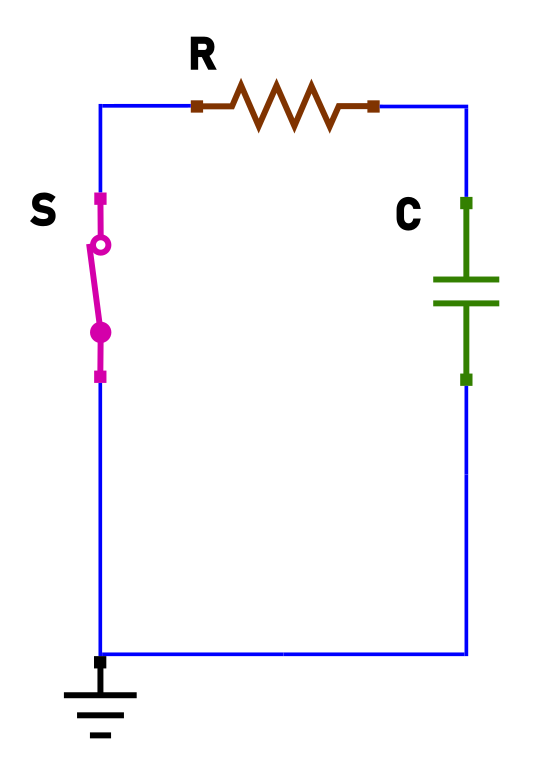
\includegraphics[width=\linewidth]{data/scarica-closed.png}
  \end{subfigure}
  \begin{subfigure}[b]{0.347\linewidth}
    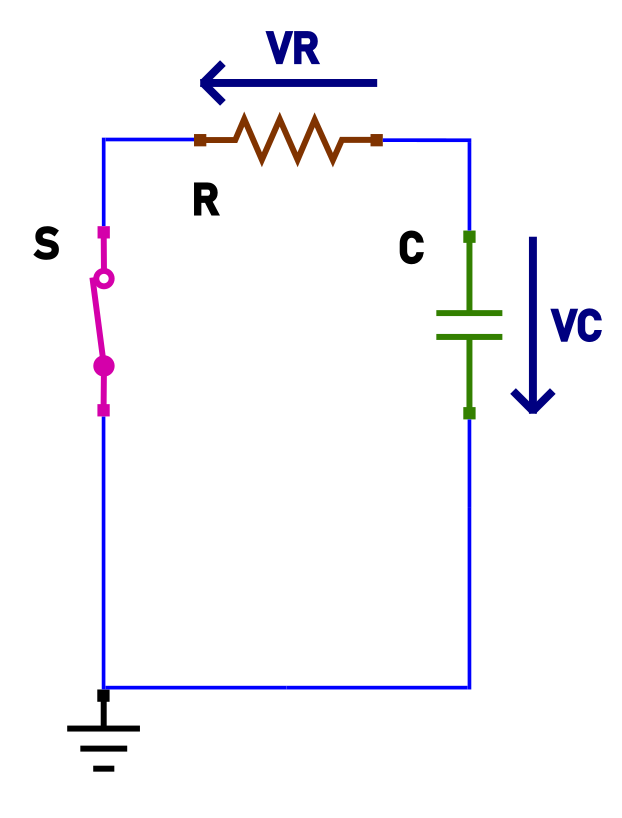
\includegraphics[width=\linewidth]{data/scarica-tensioni.png}
  \end{subfigure}
\end{figure}

Le stesse formule e regole applicate per il circuito di carica sono valide anche per il circuito di scarica. L'unica particolarità e' che nel circuito d scarica viene rimosso il generatore, e la tensione VC iniziale viene impostata a 12 V, avendo come risultato che il condensatore si comporta come un generatore.

\subsection*{grafici scarica}

\begin{figure}[h!]
  \centering
  \begin{subfigure}[b]{0.49\linewidth}
    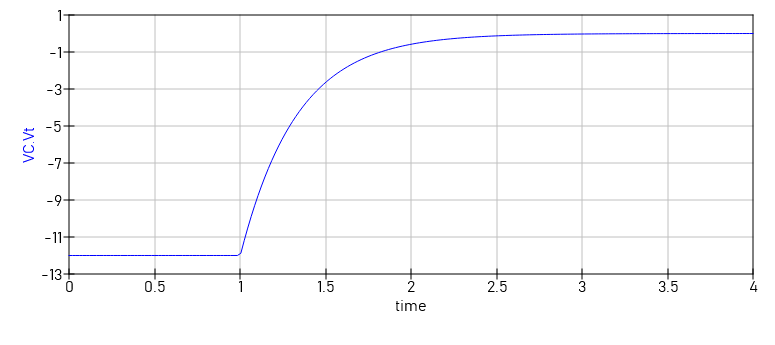
\includegraphics[width=\linewidth]{data/scarica-VC.png}
    \caption*{grafico VR}
  \end{subfigure}
  \begin{subfigure}[b]{0.49\linewidth}
    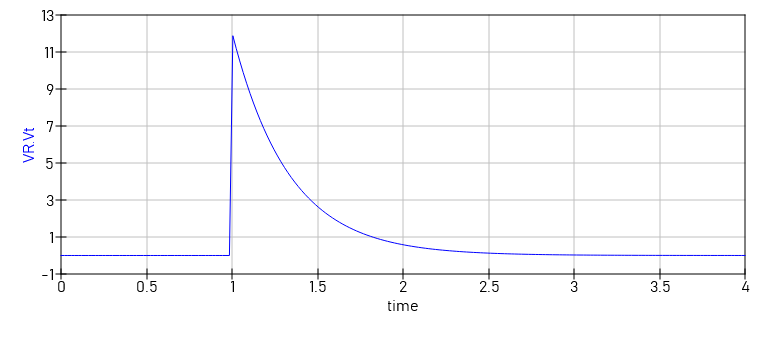
\includegraphics[width=\linewidth]{data/scarica-VR.png}
    \caption*{grafico VR}
  \end{subfigure}
  %\begin{subfigure}[b]{1\linewidth}
  %  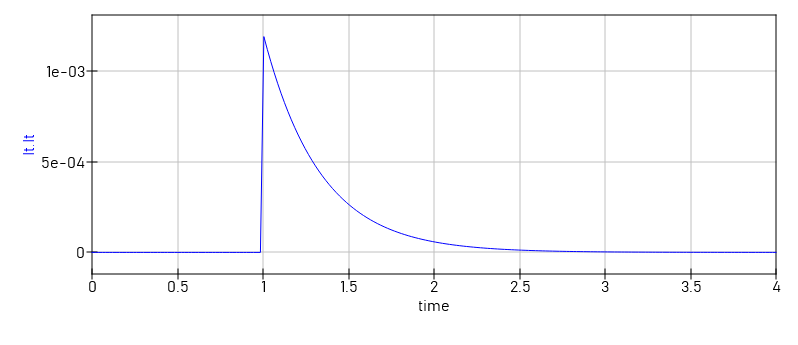
\includegraphics[width=\linewidth]{data/scarica-IT.png}
  %\end{subfigure}
\end{figure}

Per la scarica, a differenza della carica, la tensione VC e' negativa (va da -12 a 1), e la tensione VR scende anziché salire, perché, essendo il condensatore C l'unica sorgente di tensione, la tensione VR scende per il fatto che C si scarica.

\newpage

\section*{simulazione con qucs}
Gli schemi precedentemente descritti, ed i grafici ottenuti, realizzati e simulati su qucs sono riproducibili con le seguenti simulazioni:  

\subsection*{carica}

\begin{figure}[!h]
  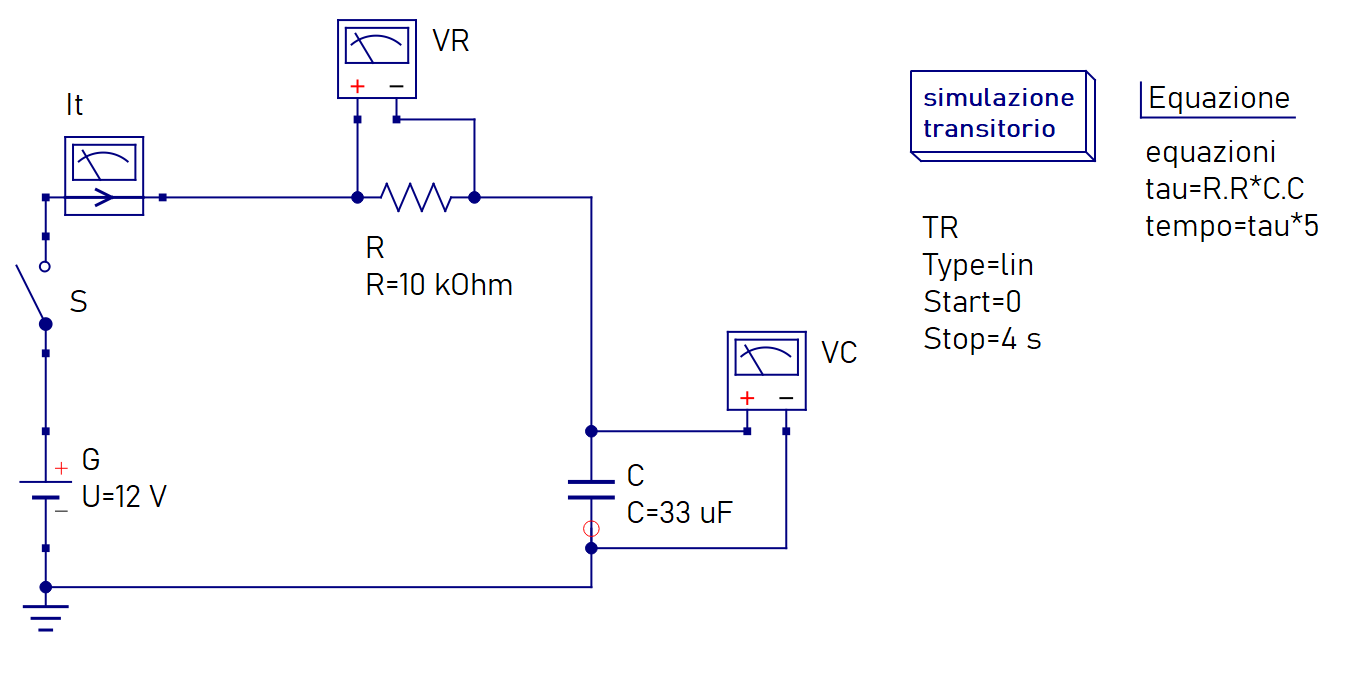
\includegraphics[width=0.9\linewidth]{data/carica-simulazione-qucs.png}
\end{figure}

\subsection*{scarica}

\begin{figure}[!h]
  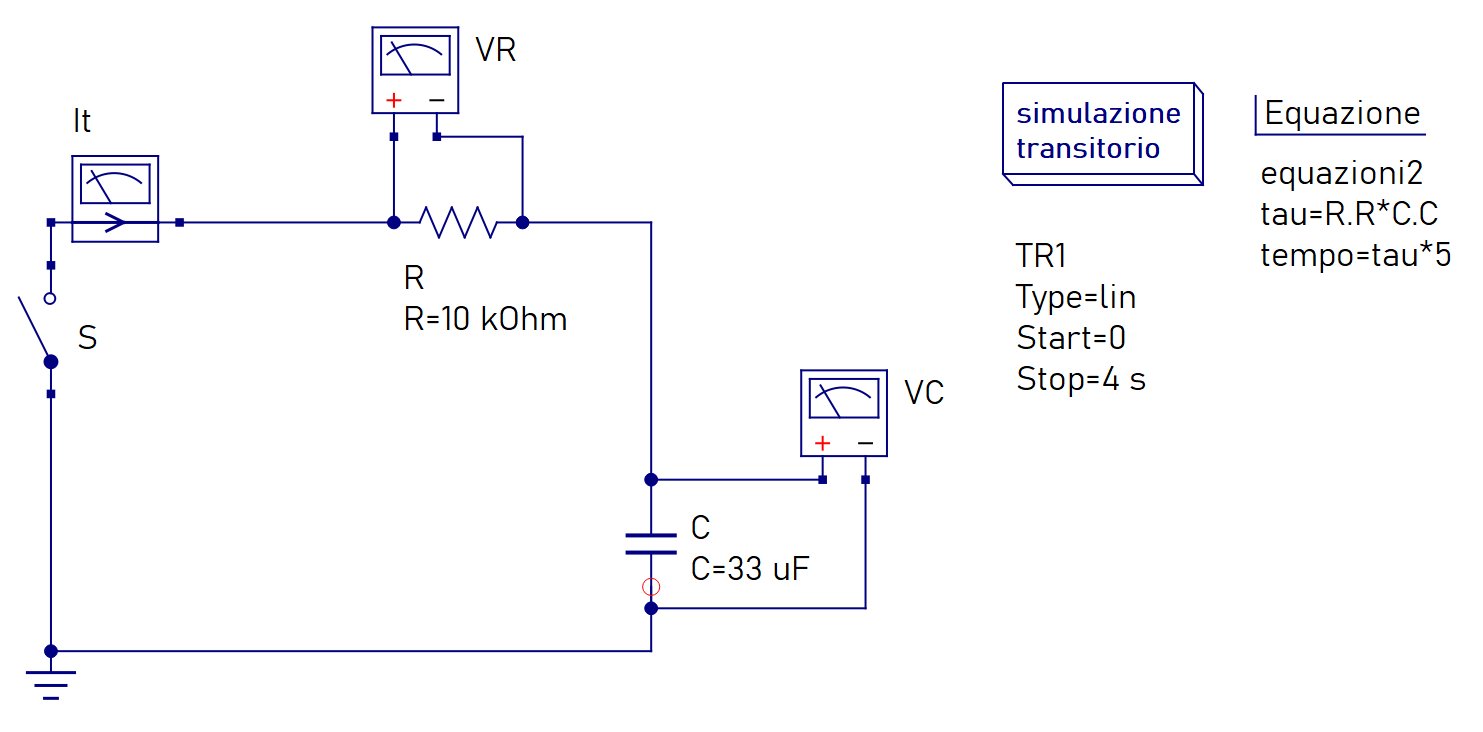
\includegraphics[width=0.9\linewidth]{data/scarica-simulazione-qucs.png}
\end{figure}

\newpage

\section*{conclusioni e osservazioni}
La simulazione del circuito, nonostante sia andata a buon fine in entrambi i casi (carica e scarica), ha prodotto un risultato inizialmente inaspettato: il voltometro, infatti, restituisce che la tensione VC ai capi del condensatore e' negativa, ciò può vuol dire che quando si scarica il condensatore i terminali cambiano potenziale (ipotesi poco probabile).
Bisogna anche considerare che abbiamo usato 2 circuiti diversi per la carica e la scarica, quindi, l'ipotesi più probabile, anzi certa, sarebbe che qucs quando deve gestire un generatore, o condensatore inizialmente carico, imposti il potenziale dei terminali sempre nello stesso orientamento, quindi, non avendo informazioni sul come si sia caricato il condensatore, esegue la simulazione con le impostazioni convenzionali. Tale ipotesi andrebbe verificata con un circuito che si occupi sia di carica che di scarica dello stesso condensatore, in modo da verificare se il comportamento di qucs e' corretto o meno.

\end{document}